\documentclass[11pt]{article}

\usepackage[T1]{fontenc}
\usepackage[utf8]{inputenc}
\usepackage{lmodern}
\usepackage{microtype}
\usepackage[margin=1in]{geometry}
\usepackage{graphicx}
\usepackage{booktabs}
\usepackage{array}
\usepackage{xcolor}
\usepackage{amsmath}
\usepackage{caption}
\usepackage{enumitem}
\usepackage{float}
\usepackage[colorlinks=true, linkcolor=blue!50!black, citecolor=blue!50!black, urlcolor=blue!50!black]{hyperref}

\newcommand{\code}[1]{\texttt{#1}}

\title{Joint Activation and Structured Sparsity\\ for ECG Arrhythmia Classification on Akida 1}
\author{Akida 1 Model Zoo}
\date{August 2026}

\begin{document}
\maketitle

\begin{abstract}
This is the fourth in a series of repeated studies on whether combining activation-sparsity regularization with structured (channel) pruning costs more, less, or the same as the sum of each mechanism's individual accuracy cost. The first three studies (Visual Wake Words, PlantVillage, Speech Commands) each found a different pattern. This report, on ECG arrhythmia classification from single-lead MIT-BIH recordings (a 1D-signal-to-scalogram task, this series' first non-image, non-audio modality), finds a fourth: activation regularization actively \emph{improves} accuracy here rather than merely costing less than expected, and the aggressive joint configuration (74.6\% activation sparsity, a 25.7\% parameter reduction) \emph{strictly dominates} a lighter alternative --- better accuracy, more sparsity, and a larger parameter cut, simultaneously, with no tradeoff to make. This is consistent with, and explained by, the companion single-axis experiment's own finding that no regularizer strength tested on this model ever caused the accuracy collapse seen in the other three studies, plausibly because this project's class-weighted loss (addressing severe class imbalance) makes the "collapse to the majority class" failure mode far less attractive here.
\end{abstract}

\tableofcontents

\section{Introduction}

This is the fourth of four repeated studies investigating the interaction between activation-sparsity regularization and structured channel pruning. The first three reached three different conclusions:

\begin{itemize}
    \item \textbf{VWW}: the joint configuration was complementary (sub-additive) throughout, and a lighter configuration simply traded some sparsity/size benefit for a smaller accuracy cost along a smooth curve.
    \item \textbf{PlantVillage}: an aggressive joint configuration was sharply antagonistic (a pruning-recovery problem), but a lighter configuration avoided this almost entirely and was a strict win on every axis.
    \item \textbf{Speech Commands}: the sign of the interaction flipped with regularization strength (complementary when aggressive, mildly antagonistic when light), and neither operating point dominated the other.
\end{itemize}

This report asks the same two questions --- does the joint cost more or less than the sum of its parts, and can a better operating point be found --- on ECG arrhythmia classification (3-class beat classification from continuous-wavelet-transform scalograms of single-lead ECG, MIT-BIH Arrhythmia Database), a fourth model, dataset, and signal modality (1D physiological time series, rather than vision or audio).

All work in this report is on the branch\\
\code{arrhythmia\_\allowbreak classification-\allowbreak joint}.
This follows up on two prior efforts: the single-axis activation-sparsity
experiment on branch \code{akida1-\allowbreak sparsify-\allowbreak arrhythmia}
(\code{SPARSITY\_EXPERIMENT.\allowbreak md}), and the joint VWW, PlantVillage,
and Speech Commands studies.

\section{Background}

\subsection{Akida 1 and activation sparsity}

Akida 1 accelerates inference by skipping computation on zero-valued activations. Structured (channel) pruning is a separate property -- how much of the model's parameter count has been physically removed -- that Akida 1's execution model does not exploit for speed; its value is reduced memory footprint.

\subsection{ECG arrhythmia classification}

The task is 3-class heartbeat classification (Normal, Supraventricular, Ventricular) from single-lead ECG recordings in the MIT-BIH Arrhythmia Database. Each heartbeat is extracted around its annotated R-peak, transformed into a continuous-wavelet-transform (CWT) scalogram image, and augmented with four rows encoding RR-interval timing features. Unlike the other three studies (two image tasks, one audio task), the raw signal here is a 1D physiological time series, and the model consumes a derived time-frequency image representation of it rather than a directly-sampled image or audio spectrogram.

\section{Dataset}

\begin{table}[H]
\centering
\caption{Dataset summary, as prepared by \code{scripts/data.py}'s \code{ECGDatasetBuilder}.}
\label{tab:dataset}
\begin{tabular}{@{}ll@{}}
\toprule
Property & Value \\
\midrule
Source & MIT-BIH Arrhythmia Database (PhysioNet), 48 records \\
Classes & 3 (N: normal, S: supraventricular, V: ventricular ectopic) \\
Class weights & $\{0: 1.0,\ 1: 6.0,\ 2: 3.0\}$ (addresses severe class imbalance) \\
Beat window & 250 samples before/after the R-peak, resampled to 360 \\
Feature transform & CWT scalogram ($32{\times}32$) + 4 RR-interval rows appended \\
Input shape & $36 \times 32 \times 1$ \\
Train / validation / test & 40{,}447 / 10{,}112 / 49{,}280 beats (stratified 80/20 train/val split) \\
\bottomrule
\end{tabular}
\end{table}

The RR-interval rows are z-scored using statistics computed from the training split only, then stacked beneath the min-max-normalized scalogram, giving each sample a real dynamic range of approximately $[-5.59, 14.83]$ -- substantially wider and more asymmetric than a naively-assumed $[-1, 1]$ or $[0, 1]$ range. (The companion single-axis experiment found and fixed a pre-existing bug where \code{scripts/eval.py} assumed the latter when converting to Akida, silently corrupting hardware-accuracy measurements; not relevant to this float-only study; see \code{SPARSITY\_EXPERIMENT.md} and \code{scripts/input\_scaling.py}.)

\section{Model architecture}
\label{sec:architecture}

The model (\code{build\_akida\_model} in \code{scripts/model.py}) is a small, custom Akida-targeted CNN: a stem convolution, two depthwise-separable blocks with max-pooling, a final depthwise-separable block without pooling or an immediately-following activation, global average pooling, and a two-layer dense classifier head. At 23,363 parameters it is the smallest of the four models studied across this series (VWW: 226,906; PlantVillage: 1,156,054; Speech Commands: 22,668 -- comparable in scale to Speech Commands, both far smaller than the two vision examples). Like the other three, it is a strict feed-forward chain with no residual/skip connections.

\begin{table}[H]
\centering
\caption{Model architecture. Every \code{*\_sepconv}/\code{stem\_conv} row is immediately followed by its own BatchNormalization (omitted for brevity; parameter counts include them). \code{block3\_bn} is notably \emph{not} followed by an activation -- the ReLU is deferred until after global average pooling.}
\label{tab:arch}
\begin{tabular}{@{}llrr@{}}
\toprule
Layer & Type & Output shape & Params (layer + BN) \\
\midrule
\code{input} & Input & $36\times32\times1$ & 0 \\
\code{stem\_conv} & Conv2D & $36\times32\times16$ & 464 \\
\code{block1\_sepconv} & SeparableConv2D & $36\times32\times32$ & 1{,}040 \\
& MaxPooling2D & $18\times16\times32$ & 0 \\
\code{block2\_sepconv} & SeparableConv2D & $18\times16\times64$ & 3{,}104 \\
& MaxPooling2D & $9\times8\times64$ & 0 \\
\code{block3\_sepconv} & SeparableConv2D (no activation) & $9\times8\times128$ & 10{,}304 \\
& GlobalAveragePooling2D & $128$ & 0 \\
& ReLU & $128$ & 0 \\
\code{dense} & Dense (linear) & $64$ & 8{,}256 \\
& ReLU & $64$ & 0 \\
\code{dense\_1} & Dense (linear, logits) & $3$ & 195 \\
\midrule
\multicolumn{3}{r}{\textbf{Total}} & \textbf{23{,}363} \\
\multicolumn{3}{r}{Trainable / non-trainable} & 22{,}883 / 480 \\
\bottomrule
\end{tabular}
\end{table}

The classifier head reads from \code{block3\_sepconv}'s output only after global average pooling and an intervening ReLU, structurally similar to the other three examples' final-feature-layer-to-classifier connection, and for the same reason: \code{block3\_sepconv} is excluded from the prunable set (Section~\ref{sec:structured}).

\section{Methodology}

The two sparsity mechanisms and the float-only rationale are identical to the prior three studies; this section highlights what differs for this project.

\subsection{Activation sparsity: normalized Hoyer-Square regularization}

The established best point from the single-axis experiment is normalized Hoyer-Square at $\lambda=3$: 68.2\% activation sparsity (Akida-measured) for only a $\sim$0.9-point accuracy cost from the unregularized baseline -- the cheapest sparsity gain of any of the four model-zoo examples studied. Uniquely among the four, this project's single-axis sweep found \textbf{no regularizer strength that caused a training collapse}, even at 30--100$\times$ the strengths that fully destroyed VWW's, PlantVillage's, and Speech Commands' accuracy -- attributed in \code{SPARSITY\_EXPERIMENT.md} to the class-weighted loss (Table~\ref{tab:dataset}) making "predict only the majority class" a much less attractive failure mode here.

\subsection{Structured sparsity: Network Slimming, located positionally}
\label{sec:structured}

Network Slimming \cite{networkslimming} is applied via \code{scripts/arrhythmia\_structured\_sparsity.py}, adapted from the VWW implementation with one change: this project's BatchNormalization layers are named \code{\{block\}\_bn} (e.g.\ \code{block1\_bn}) rather than \code{\{layer\}/BN}. Rather than hardcoding yet another naming convention, the paired BN is now located \emph{positionally} -- the layer immediately following the target in \code{model.layers} -- a more robust approach in general, since it makes no assumption about naming at all. \textbf{Pruning scope}: \code{block1\_sepconv} and \code{block2\_sepconv} (2 of this model's 3 SeparableConv2D blocks); \code{block3\_sepconv} is excluded since it feeds the classifier head directly. This model has only 3 SeparableConv2D blocks total (versus VWW's and PlantVillage's 10, Speech Commands' 4), so its prunable set is smaller by construction than any of the other three.

\subsection{Float-only evaluation}

As with the other three studies, no \code{cnn2snn quantize}/QAT/\code{convert} is used anywhere in this pipeline. Activation sparsity is the mean fraction of exactly-zero ReLU outputs on 1{,}000 held-out samples, and is \textbf{not directly comparable} to the single-axis experiment's Akida-measured figures for the same reason as the other three studies.

\subsection{Training pipeline}

Unlike VWW, PlantVillage, and Speech Commands -- each of which exposes a reusable \code{train\_*(model, ...)} function that this series' sweep scripts import directly -- this project's \code{scripts/train.py} runs float training, quantization, and QAT all inline in a single \code{\_\_main\_\_} script, with no importable training function. This report's sweep instead calls \code{build\_akida\_model}/\code{apply\_activity\_regularizer} directly and implements its own simple training loop (float-only, so no quantize/QAT stage is needed regardless).

\paragraph{Best-checkpoint reload.} \code{train.py}'s own convention is \code{ModelCheckpoint(monitor="val\_loss", save\_best\_only=True)} together with \code{EarlyStopping(patience=8, restore\_best\_weights=False)} -- meaning the live in-memory model immediately after \code{fit()} is \emph{not} necessarily the best one seen during training. This report's training loop reproduces that exactly, reloading the checkpointed best-val-loss model after every training phase.

\begin{description}
    \item[Phase 1 (float training, up to 80 epochs).] Matches \code{train.py}'s float-training scale (Adam, learning rate $3\times10^{-3}$, \code{ReduceLROnPlateau} and \code{EarlyStopping(patience=8)} -- so 80 is a ceiling, not a fixed count).
    \item[Pruning (if $p>0$).] Channels pruned per Section~\ref{sec:structured}.
    \item[Phase 2 (post-prune fine-tuning, up to 40 epochs, learning rate $3\times10^{-4}$).] Only run when $p>0$.
\end{description}

The class-weighted loss $\{0{:}1.0,\ 1{:}6.0,\ 2{:}3.0\}$ (pre-existing, addressing this dataset's severe class imbalance) is applied unchanged in every phase.

\paragraph{Training speed.} At 23,363 parameters and small $36\times32\times1$ inputs, each epoch takes roughly 5--7 seconds on GPU~1 of the shared training server. Despite the two-phase-with-fine-tuning structure, the full pilot (4 configurations) and follow-up (3 more) together completed in well under 20 minutes.

\section{Experimental design}

\paragraph{Pilot (2$\times$2 grid).} All four combinations of activation regularization on/off ($\lambda=3$, the established best single-axis point) and pruning on/off ($p=40\%$, a starting guess mirroring the other three studies' choice on this axis).

\paragraph{Follow-up (lighter settings).} Three lighter points, halving both knobs: $\lambda=1.5$ and $p=20\%$, individually and jointly.

\begin{table}[H]
\centering
\caption{All configurations run. $\lambda$ is the normalized Hoyer-Square strength; $p$ is the structured prune target.}
\label{tab:configs}
\begin{tabular}{@{}lrr@{}}
\toprule
Tag & $\lambda$ & $p$ \\
\midrule
\code{baseline} & 0 & 0\% \\
\code{activation\_only} & 3 & 0\% \\
\code{structured\_only} & 0 & 40\% \\
\code{joint} & 3 & 40\% \\
\code{activation\_light} & 1.5 & 0\% \\
\code{structured\_light} & 0 & 20\% \\
\code{joint\_light} & 1.5 & 20\% \\
\bottomrule
\end{tabular}
\end{table}

\section{Results}
\label{sec:results}

\begin{table}[H]
\centering
\caption{Full results. Accuracy drop is relative to \code{baseline} (93.85\%); a \emph{negative} drop means the configuration outperformed baseline. Parameter reduction is relative to \code{baseline}'s 23{,}363 parameters. Activation sparsity is the float-model measurement and is \emph{not} directly comparable to the single-axis experiment's Akida-measured numbers.}
\label{tab:results}
\begin{tabular}{@{}lrrrrrr@{}}
\toprule
Tag & $\lambda$ & $p$ & Accuracy & Acc.\ drop & Act.\ sparsity & Params (reduction) \\
\midrule
\code{baseline}          & 0   & 0\%  & 93.85\% & --      & 48.7\% & 23{,}363 (--) \\
\code{activation\_only}  & 3   & 0\%  & 95.26\% & $-$1.41pt & 79.2\% & 23{,}363 (0\%) \\
\code{activation\_light} & 1.5 & 0\%  & 93.73\% & 0.12pt  & 73.0\% & 23{,}363 (0\%) \\
\code{structured\_only}  & 0   & 40\% & 93.44\% & 0.41pt  & 45.5\% & 17{,}370 (25.7\%) \\
\code{structured\_light} & 0   & 20\% & 93.35\% & 0.50pt  & 47.3\% & 20{,}330 (13.0\%) \\
\code{joint}             & 3   & 40\% & \textbf{94.43\%} & $\mathbf{-0.57pt}$ & \textbf{74.6\%} & \textbf{17{,}370 (25.7\%)} \\
\code{joint\_light}      & 1.5 & 20\% & 94.01\% & $-$0.15pt & 70.8\% & 20{,}330 (13.0\%) \\
\bottomrule
\end{tabular}
\end{table}

\begin{figure}[H]
    \centering
    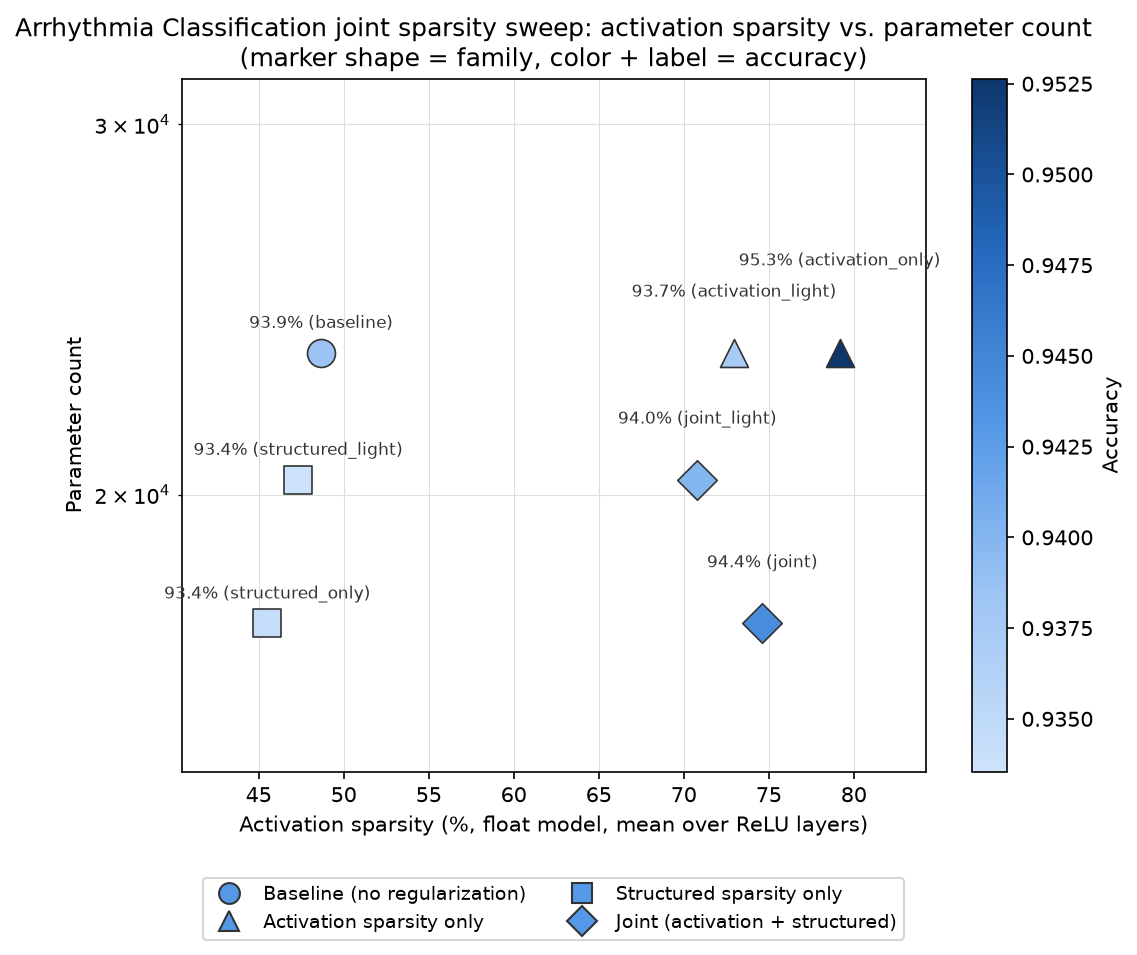
\includegraphics[width=0.85\textwidth]{joint_sparsity_sweep.png}
    \caption{Activation sparsity vs.\ parameter count for all seven configurations. Marker shape encodes family (circle: baseline, triangle: activation sparsity only, square: structured sparsity only, diamond: joint); marker color and the accompanying label encode accuracy.}
    \label{fig:sweep}
\end{figure}

\subsection{Activation regularization improves accuracy here, not just sparsity}

\code{activation\_only} beats \code{baseline} by 1.41 accuracy points (93.85\% $\to$ 95.26\%) while simultaneously gaining 30.5 points of activation sparsity. This matches the single-axis experiment's own finding of non-monotonic, sometimes-\emph{improving} accuracy as a function of regularizer strength on this dataset, attributed there to the class-weighted loss making mild regularization act as a generalization aid rather than a pure capacity reduction. None of VWW, PlantVillage, or Speech Commands showed this behavior -- every activation regularizer tested on those three cost at least some accuracy.

\subsection{The joint configuration also beats baseline}

\code{joint} reaches 94.43\% accuracy (a 0.57-point \emph{gain} over baseline) with 74.6\% activation sparsity and the full 25.7\% parameter reduction \code{structured\_only} achieves alone. Structured pruning's own small cost (\code{structured\_only}: 0.41pt) is more than offset when combined with activation regularization's accuracy gain.

\subsection{A fourth distinct pattern: the aggressive configuration strictly dominates the light one}

Unlike all three prior studies -- where the lighter joint configuration either simply cost less (VWW), was a strict win on every axis (PlantVillage), or traded one axis for another with neither point dominating (Speech Commands) -- here \code{joint} beats \code{joint\_light} on \emph{every} axis simultaneously: higher accuracy (94.43\% vs.\ 94.01\%), higher activation sparsity (74.6\% vs.\ 70.8\%), and a larger parameter reduction (25.7\% vs.\ 13.0\%). There is no tradeoff to make between these two points; pushing both regularization knobs harder simply helped, within the range tested.

\subsection{Consistent with this project's own collapse-free single-axis behavior}

This finding is not an isolated anomaly: it is consistent with \code{SPARSITY\_EXPERIMENT.md}'s own observation that no regularizer type or strength tested on this model ever produced the accuracy collapse the other three projects' sweeps all eventually hit, even at 30--100$\times$ the strength that destroyed those models. If stronger regularization/pruning simply keeps paying off up to some much higher strength than tested here, that would explain why the aggressive joint corner in this pilot has not yet found a downside.

\section{Discussion and limitations}

\paragraph{Has the ceiling been found?} Since \code{joint} dominates \code{joint\_light} rather than trading against it, and given the single-axis experiment's own note that this model's collapse point (if one exists) lies well beyond anything tested so far, it is plausible that pushing $\lambda$ and/or $p$ even higher than this pilot's ``aggressive'' corner would continue to help. A follow-up sweep at, e.g., $\lambda=10$ and $p=60\%$ would test whether the dominance pattern holds further out or eventually reverses.

\paragraph{This dataset's noise floor warrants caution.} \code{SPARSITY\_EXPERIMENT.md} documented non-monotonic, seed-sensitive results throughout its own sweep on this small, heavily-imbalanced dataset (49,280 test beats, but very few training examples for the minority S and V classes). The accuracy \emph{gains} reported here are plausible and mechanistically explicable, but have not been confirmed across multiple random seeds -- a single training run's ranking between closely-spaced configurations should not yet be treated as a firm conclusion.

\paragraph{Float-vs-hardware sparsity gap and no latency validation.} As with the other three studies, the float-model sparsity measurements here are not on the same footing as the single-axis experiment's Akida-hardware/software-simulator-measured figures, and this report makes no claim about actual Akida 1 latency or power.

\section{Conclusion}

Repeating the joint activation-sparsity and structured-sparsity investigation a fourth time, on ECG arrhythmia classification, produced yet another distinct pattern from VWW, PlantVillage, and Speech Commands. Activation regularization measurably \emph{improves} accuracy on this dataset rather than merely costing less than expected, and the aggressive joint configuration ($\lambda=3$, 40\% pruning) strictly dominates a lighter alternative on every axis tested -- accuracy, activation sparsity, and parameter count all improve together, with no tradeoff to navigate. This traces to a property specific to this dataset and its class-weighted training loss: unlike the other three examples, no regularizer strength tested here has ever caused a training collapse, so pushing harder within the tested range simply keeps paying off. Across all four studies now completed, the overarching lesson holds: the interaction between activation-sparsity regularization and structured pruning is model- and dataset-specific in ways that range from complementary to antagonistic to (as seen here) unambiguously beneficial, and must be measured directly for each new model rather than assumed from any prior result.

\begin{thebibliography}{9}

\bibitem{networkslimming}
Z.~Liu, J.~Li, Z.~Shen, G.~Huang, S.~Yan, and C.~Zhang.
\newblock Learning Efficient Convolutional Networks through Network Slimming.
\newblock In \emph{Proceedings of the IEEE International Conference on Computer Vision (ICCV)}, 2017.

\bibitem{deephoyer}
H.~Yang, W.~Wen, and H.~Li.
\newblock DeepHoyer: Learning Sparser Neural Network with Differentiable Scale-Invariant Sparsity Measures.
\newblock In \emph{International Conference on Learning Representations (ICLR)}, 2020.

\bibitem{mitbih}
G.~B.~Moody and R.~G.~Mark.
\newblock The Impact of the MIT-BIH Arrhythmia Database.
\newblock \emph{IEEE Engineering in Medicine and Biology Magazine}, 20(3):45--50, 2001.

\end{thebibliography}

\end{document}
